% I removed the definition of a manifold and moved it in-line for better flow.
% I think it's best to use /emph in definitions to show what's being defined.
% Put periods even in display math!
% For spacing reasons, should use \colon instead of : for functions, e.g. f \colon A \to B.
% Since ker is lowercase, im probably should be also.

\section{Introduction: singular simplices and chains}\label{905}
This is a course on algebraic topology. 
We'll discuss the following topics. 
\begin{enumerate}
    \item Singular homology
    \item CW-complexes
    \item Basics of category theory
    \item Homological algebra
    \item The K\"{u}nneth theorem
    \item Universal coefficient theorems, cohomology
    \item Cup and cap products
    \item Poincar\'{e} duality.
\end{enumerate}
The objects of study are of course topological spaces, and the machinery
we develop in this course is designed to be applicable to a general space. 
But we are really interested in geometrically important spaces. Here are 
some examples. 
\begin{itemize}
    \item The most basic example is \emph{$n$-dimensional Euclidean space}, $\mathbf{R}^n$.
    \item The \emph{$n$-sphere} $S^n=\{x\in \mathbf{R}^{n+1}:|x|=1\}$, topologized as a subspace of $\mathbf{R}^{n+1}$.
    \item Identifying antipodal points in $S^n$ gives \emph{real projective space} $\mathbf{RP}^n=S^n / (x\sim -x)$, i.e. the space of lines through the origin in $\mathbf{R}^{n+1}$.
    \item Call an ordered collection of $k$ orthonormal vectors an \emph{orthonormal $k$-frame}. The space of orthonormal $k$-frames in $\mathbf{R}^n$ forms the \emph{Stiefel manifold} $V_k(\mathbf{R}^n)$, which is topologized as a subspace of $(S^{n-1})^k$.
   \item The \emph{Grassmannian}  $\mathrm{Gr}_k(\mathbf{R}^n)$ is the space of
$k$-dimensional linear subspaces of $\mathbf{R}^n$. Forming the span gives us
a surjection $V_k(\mathbf{R}^n)\to\mathrm{Gr}_k(\mathbf{R}^n)$, and the
Grassmannian is given the quotient topology. 
For example, $\mathrm{Gr}_1(\mathbf{R}^n) = \mathbf{RP}^{n-1}$.
\end{itemize}
All these examples are \emph{manifolds}; that is, they are Hausdorff spaces locally homeomorphic to Euclidean space. Aside from $\mathbf{R}^n$ itself, the preceding examples are also compact. Such spaces exhibit a hidden symmetry, which is the culmination of 18.905: Poincar\'{e} duality.

As the name suggests, the central aim of algebraic topology is the usage of algebraic tools to study topological spaces. A common technique is to probe topological spaces via maps to them from simpler spaces. In different ways, this approach gives rise to singular homology and homotopy groups. We now detail the former; the latter takes the stage in 18.906.
\begin{definition}
For $n\geq 0$, the \emph{standard $n$-simplex} $\Delta^n$ is the convex hull of the standard basis $\{e_0,\ldots,e_n\}$ in $\mathbf{R}^{n+1}$:
$$\Delta^n = \left\{\sum t_i e_i : \sum t_i = 1, t_i\geq 0\right\}\subseteq\mathbf{R}^{n+1}.$$
The $t_i$ are called {\em barycentric coordinates}.
\end{definition}
%We will write $i$ in lieu of $e_i$ to refer to the vertices of $\Delta^n$. 
The standard simplices are related by face inclusions $d^i\colon \Delta^{n-1} \to \Delta^{n}$ for $0\leq i \leq n$, where $d^i$ is the affine map that sends
verticies to vertices, in order, and omits the vertex $e_i$.

\begin{center}
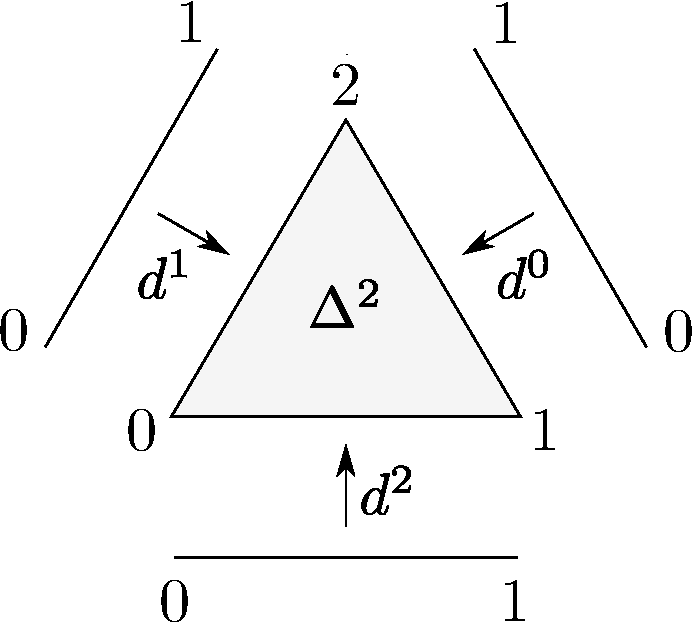
\includegraphics[width=3in]{905/Figures/01-2-simplex.pdf}
\end{center}

\begin{definition}
Let $X$ be any topological space. A \emph{singular $n$-simplex} in $X$ is a continuous map $\sigma:\Delta^n\to X$. Denote by $\mathrm{Sin}_n(X)$ the set of all $n$-simplices in $X$.
\end{definition}
    
This seems like a rather bold construction to make, as $\mathrm{Sin}_n(X)$ is huge. But be patient! 

For $0\leq i \leq n$, precomposition by the face inclusion $d^i$ produces a map $d_i\colon \Sin_n(X)\to\Sin_{n-1}(X)$ sending $\sigma\mapsto\sigma\circ d^i$. This is the ``$i$th face'' of $\sigma$. This allows us to make sense of the ``boundary'' of a simplex, and we are particularly interested in simplices for which that boundary vanishes.

For example, if $\sigma$ is a 1-simplex that forms a closed loop,
then $d_1\sigma = d_0\sigma$. To express the condition that the boundary vanishes, we would like to write $d_0\sigma - d_1\sigma=0$ -- but this difference is no longer a simplex. To accommodate such formal sums, we will enlarge $\mathrm{Sin}_n(X)$ further by forming the free abelian group it generates.
\begin{definition}
The abelian group $S_n(X)$ of \emph{singular $n$-chains} in $X$ is the free abelian group generated by $n$-simplices
$$S_n(X) = \mathbf{Z}\Sin_n(X).$$
\end{definition}
So an $n$-chain is a finite linear combination of simplices,
\[
\sum_{i=1}^ka_i\sigma_i\,,\quad a_i\in\mathbf{Z}\,,\quad\sigma_i\in\Sin_n(X)\,.
\]
If $n<0$, $\Sin_n(X)$ is declared to be empty, so $S_n(X)=0$. 

We can now define the {\em boundary operator}
$$d\colon \Sin_n(X)\to S_{n-1}(X),$$
by
$$d\sigma = \sum_{i=0}^n(-1)^i d_i\sigma.$$
This extends to a homomorphism $d \colon S_n(X) \to S_{n-1}(X)$ by additivity.

We use this homomorphism to obtain something more tractable than the entirety of $S_n(X)$. First we restrict our attention to chains with vanishing boundary.
\begin{definition}
An \emph{$n$-cycle} in $X$ is an $n$-chain $c$ with $dc = 0$. Notation:
\[
Z_n(X) = \ker(d:S_n(X)\rightarrow S_{n-1}(X))\,.
\]
\end{definition}
For example, if $\sigma$ is a $1$-simplex forming a closed loop, then 
$\sigma\in Z_1(X)$ since $d\sigma = d_0\sigma - d_1\sigma = 0$.

It turns out that there's a cheap way to produce a cycle:
\begin{theorem}
    Any boundary is a cycle; that is, $d^2=0$.
\end{theorem}
We'll leave the verification of this important result as a homework problem. 
What we have found, then, is that the singular chains form a ``chain complex,''
as in the following definition.
\begin{definition}
A {\em graded abelian group} is a sequence of abelian groups, indexed by 
the integers. 
A {\em chain complex} is a graded abelian group $\{A_n\}$ together with 
homomorphisms $d:A_n\to A_{n-1}$ with the property that $d^2=0$.
\end{definition}

The group of $n$-dimensional {\em boundaries} is 
\[
B_n(X) = \img(d:S_{n+1}(X)\to S_n(X))\,,
\]
and the theorem tells us that this is a subgroup of the group of cycles: the
``cheap'' ones. If we quotient by them, what's left is the ``interesting 
cycles,'' captured in the following definition.
\begin{definition}
The \emph{$n$th singular homology group} of $X$ is:
\[
H_n(X) = \frac{Z_n(X)}{B_n(X)} = \frac{\ker(d:S_n(X)\to S_{n-1}(X))}{\img(d:S_{n+1}(X)\to S_n(X))}\,.
\]
\end{definition}
We use the same language for any chain complex: it has cycles, boundaries, and
homology groups. The homology forms a graded abelian group. 

Both $Z_n(X)$ and $B_n(X)$ are free abelian groups because they are subgroups of the free abelian group $S_n(X)$, but the quotient $H_n(X)$ isn't necessarily free. While $Z_n(X)$ and $B_n(X)$ are uncountably generated, $H_n(X)$ turns out to be finitely generated for the spaces we are interested in. If $T$ is the torus, for example, then we will see that $H_1(T) \cong \mathbf{Z} \oplus \mathbf{Z}$, with generators given by the 1-cycles illustrated below. 

\begin{center}
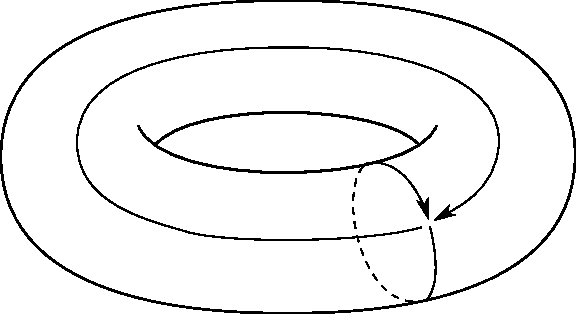
\includegraphics[width=3in]{905/Figures/01-torus-generating-cycles}
\end{center}

We will learn to compute the homology groups of a wide variety of spaces. 
The $n$-sphere for example has the following homology groups:
\[
H_q(S^n)=\begin{cases}\ZZ & \hbox{if}\quad q=n>0\\
                \ZZ & \hbox{if}\quad q=0,n>0\\
                \ZZ\oplus\ZZ & \hbox{if}\quad q=n=0\\
                0 & \hbox{otherwise}\,.
\end{cases}
\]





